\documentclass{beamer}
\usetheme{default}

\usepackage{caption}
\usepackage{subcaption}

\title{1m structure method: time-resolved x-ray scattering and photoelectron spectroscopy}
\author{T.\ Northey}
\date{4 Oct 2022 group meeting}
\begin{document}
\begin{frame}[plain]
    \maketitle
\end{frame}

\begin{frame}
	% start the columns environment    
	\begin{columns} 
		% Column 1
		\begin{column}{.4\textwidth}
			\begin{figure}[H]
				\centering
				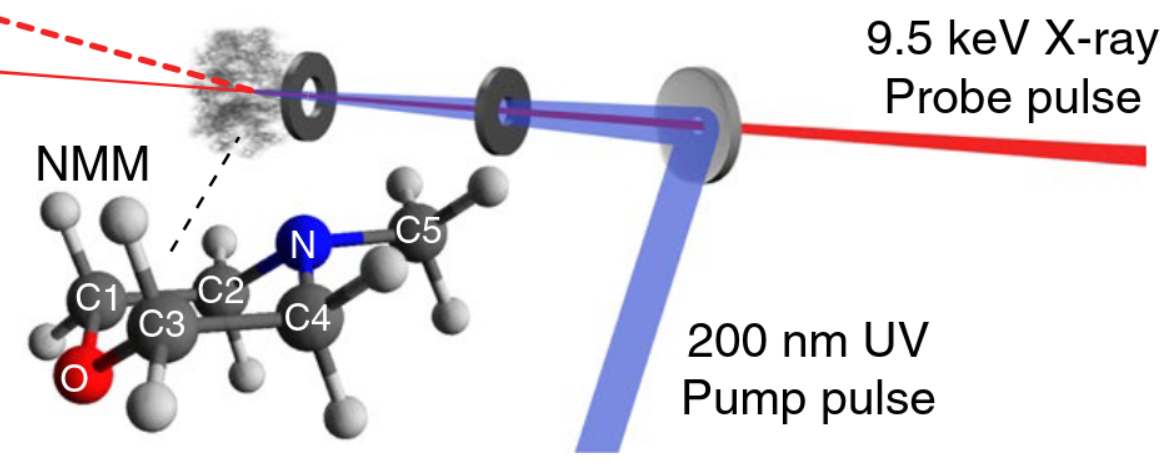
\includegraphics[width=\textwidth]{nmm_geometry.png}
				\caption{NMM geometry, and experimental setup.}
				\label{fig:nmm-geom}
			\end{figure}
		\begin{itemize}
			
			\item 107 surface hopping trajectories (1000 fs), $\sim$$10^6$ molecular geometries 
			
		\end{itemize}
		{\tiny B.\ Stankus, et al.\ Nature Chem.\ 11.8 (2019):\ 716-721.}
		\end{column}
		% Column 2    
		\begin{column}{.6\textwidth}
			\begin{figure}[H]
				\centering
				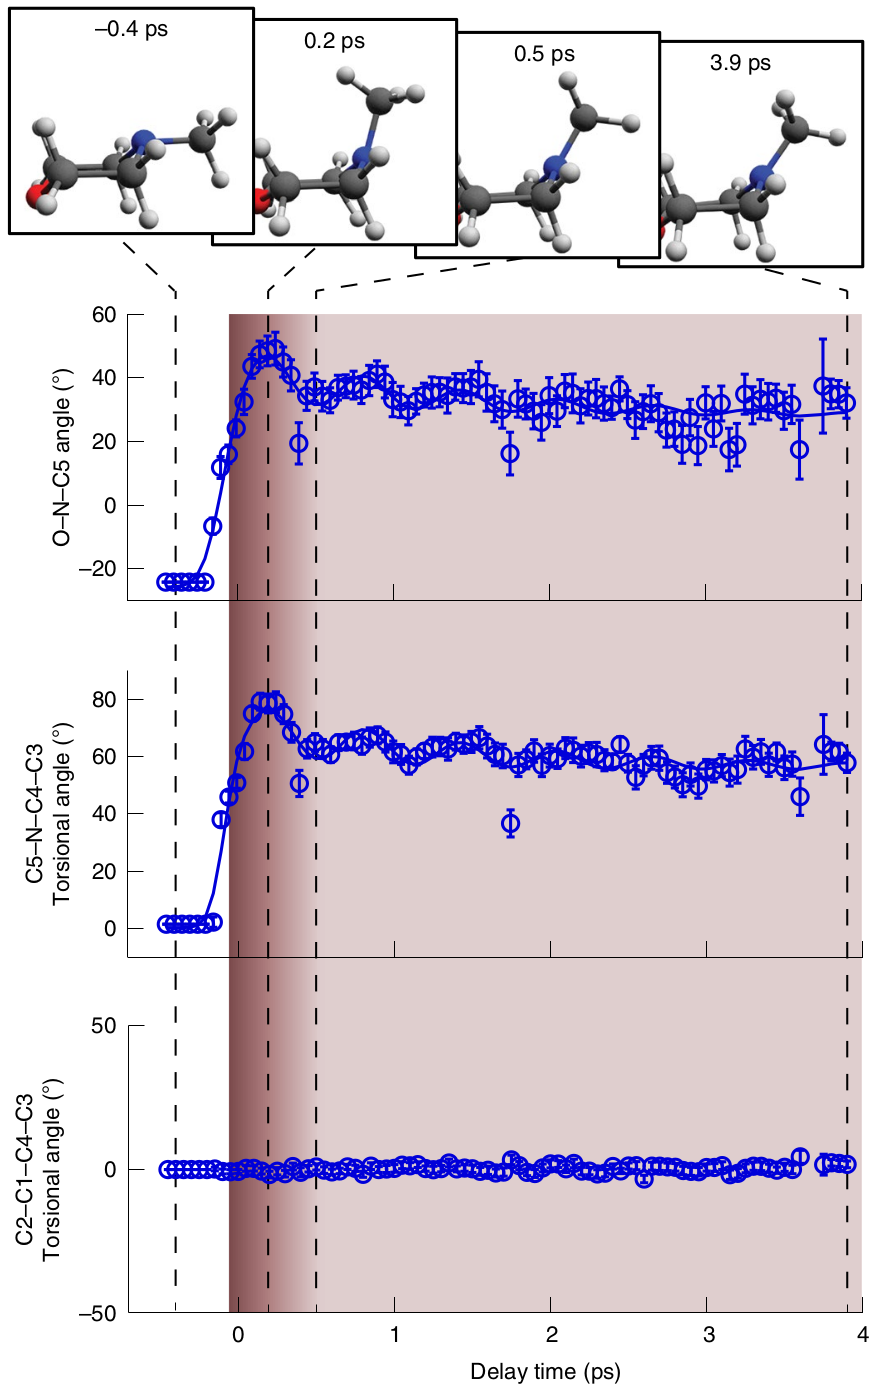
\includegraphics[width=0.7\textwidth]{stankus_angle_plots.png}
				\caption{Time-dependent angle plots
					following Rydberg excitation.}
				\label{fig:nmm-geom}
			\end{figure}
		\end{column}%
		
	\end{columns}
\end{frame}

\begin{frame}
	% start the columns environment    
	\begin{columns} 
		% Column 1
		\begin{column}{.5\textwidth}
			\begin{itemize}

				\item 107 surface hopping trajectories (1,000 fs), giving $\sim$$10^6$ molecular geometries 
				
			\end{itemize}
		\end{column}
		% Column 2    
		\begin{column}{.5\textwidth}

		\end{column}%
		
	\end{columns}
\end{frame}

\begin{frame}{Defining structure pool parameters}
\begin{center}
	{\huge$\mu$}\qquad\qquad{\huge$\sigma_i$}\\
	\vspace{2cm}
	{\huge$\rho$}
\end{center}
\end{frame}

\begin{frame}{Defining structure pool parameters}
	\begin{center}

	\end{center}
\end{frame}

\begin{frame}{Defining structure pool parameters}
		\begin{center}
	{\huge$\mu=0$, e.g.\ $\textbf{R}_0$}
		\end{center}
	
	[picture of potential energy curve along a bond-distance, + bell curve vibrational distribution]
	
	[and picture of $\mu\neq 0$ situation, shifted bell curve]
\end{frame}

\begin{frame}{Defining structure pool parameters}
		\begin{center}
	$\sigma=\begin{pmatrix}
	0.4 \\
	0.2\\
	0.2\\
	\vdots\\
	0.2
	\end{pmatrix}
	$ \AA
		\end{center}
	
	\begin{itemize}
		\item some displacements more important than others
		\item some could be irrelevant $\sigma_i = 0$ (i.e.\ don't displace at all)
	\end{itemize}

\end{frame}

\begin{frame}{Defining structure pool parameters}
		\begin{center}
	\qquad\qquad\qquad\ \ \ {\huge$\rho\propto\textrm{accuracy / resolution}$}\\
		\vspace{2mm}
	{\huge$\propto N$}\\
		\vspace{2mm}
	\quad\ \ {\huge$\propto 1/\sigma_i$}\\
	%\qquad\qquad\qquad\ \ {\huge$\propto 1/n_{\textrm{modes}}$}\\

		\end{center}

\end{frame}

\begin{frame}{NMM previous work}
	\begin{figure}[H]
		\centering
		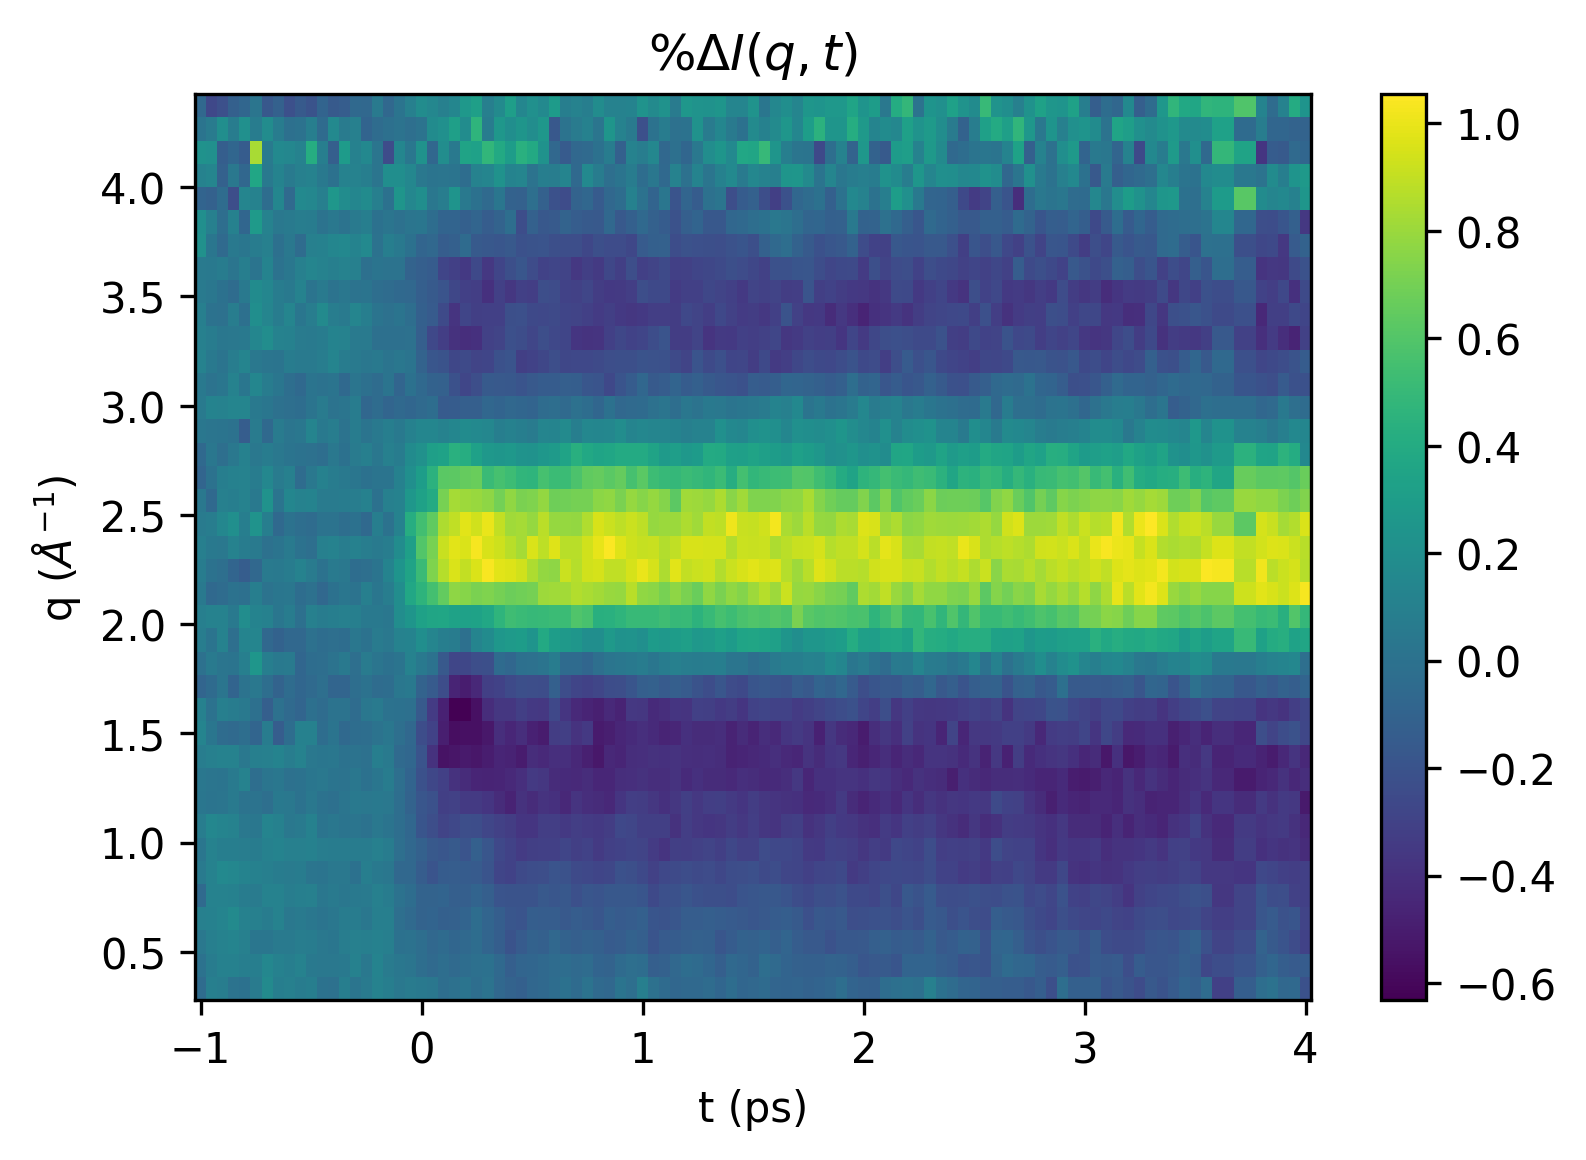
\includegraphics[width=0.6\textwidth]{NMM_exp_2Dplot.png}
		\caption{Time-resolved x-ray scattering percent difference signal for NMM.}
		\label{fig:nmm-2dplot}
	\end{figure}
\vspace{-5mm}
	\begin{itemize}
		\item $q = [0.33, 4.37] $ \AA$^{-1}$, (with 39 $q$-bins)
		\item Excitation percentage, 5.7\%
		\item Maximum signal difference $\simeq 1\%$
	\end{itemize}
\end{frame}

\begin{frame}{NMM previous work}
	\begin{figure}[H]
	\centering
		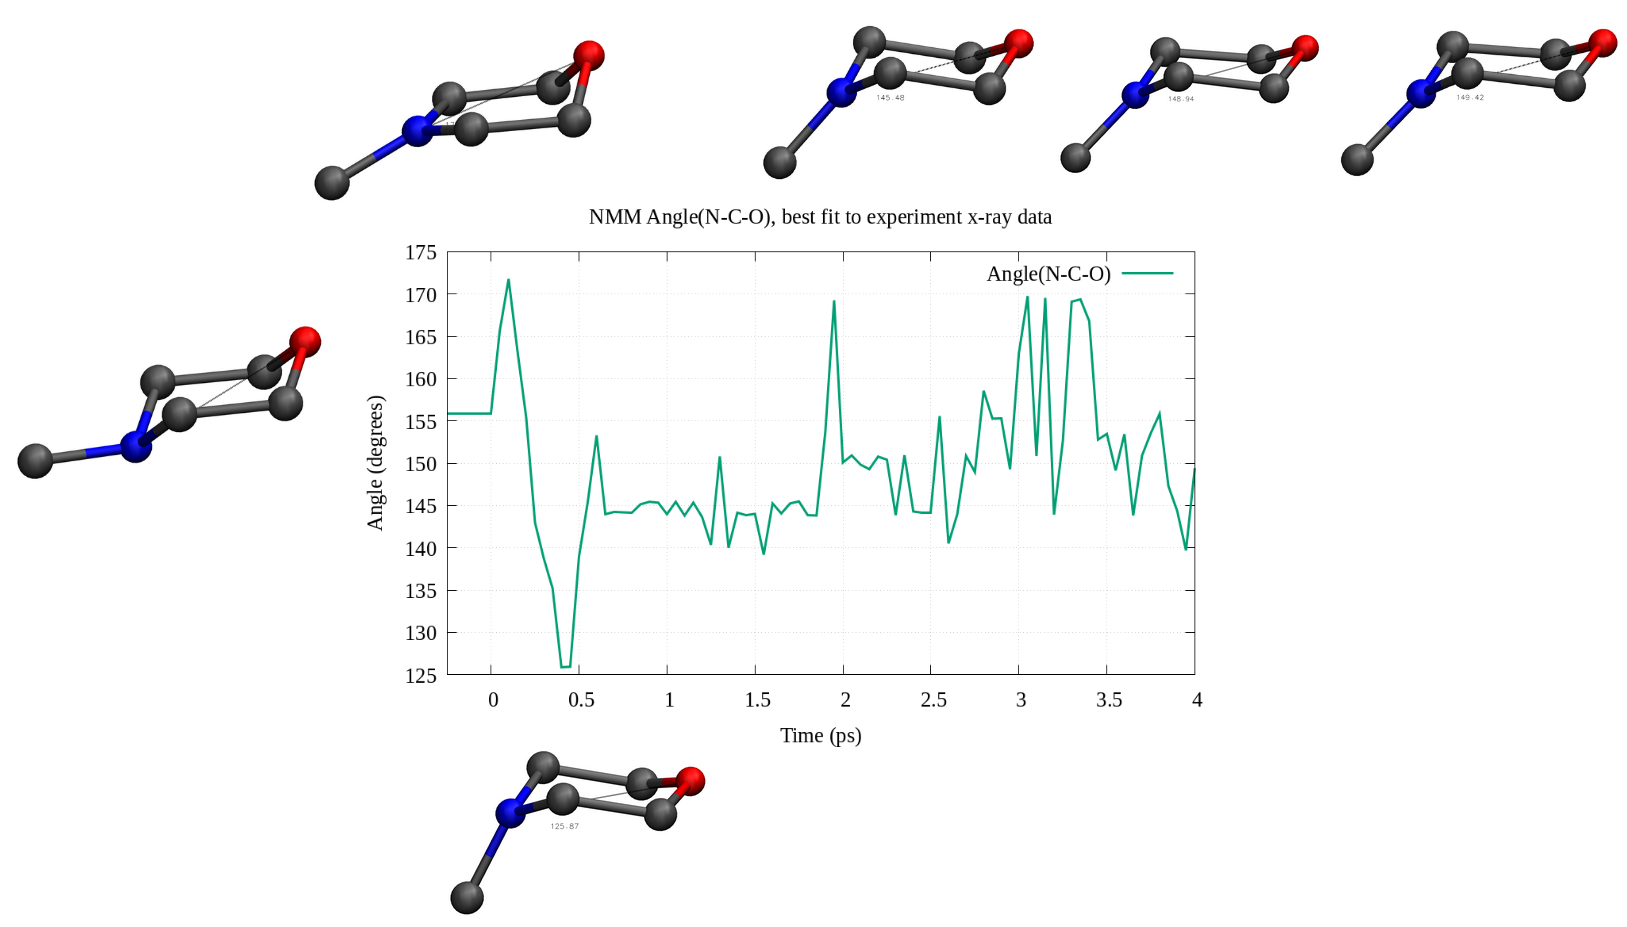
\includegraphics[width=\textwidth]{geomovie_ppt_slide.png}
		\caption{N-C-O angle, best fit to experiment x-ray data.}
		\label{fig:geomovie-ppt-slide}
	\end{figure}

\end{frame}


\begin{frame}{Sampling method}
The sampling equation for generating the displaced molecular coordinates is,

\begin{eqnarray}
\textbf{R} = \textbf{R}_0 + \sum_i^{\textrm{modes}} a_i\textbf{d}_i
\end{eqnarray}

with starting geometry $\textbf{R}_0$, and displacement unit vectors $\textbf{d}_i$ for each normal mode are obtained from a frequency calculation.  The factors $a_i$ are randomly generated within a bell curve centered at $\mu=0$, and chosen standard deviation, $\sigma$. 
\end{frame}


\end{document}
